\subsection{Simulação 2 - Simulação completa}

Após a avaliação das extremidades da pá, deve-se ainda simular o revestimento
total, pois a superfície da pá é muito irregular, podendo se aproximar ou se
afastar do robô para certas posições de base. Além disso, foram abordadas novas
estratégias para a solução de revestimento da extremidade direita da pá. A
simulação de teste de toda a pá considerou as seguintes variáveis:

\begin{itemize}
  \item O ângulo das pás da turbina variam de $0^o$ a $24^o$. O acréscimo deste
  grau de liberdade buscou solucionar o problema da extremidade direita.
  \item O rotor da turbina foi girado de $0^o$ a $30^o$ com passo de $3^o$.
  Manteve-se este grau de liberdade, pois em conjunto com o giro da pá, o
  problema da extremidade superior direita poderia ser solucionado.
  \item A distância entre extremidade da pistola e pá pode variar $235
  \pm 5$ mm.
  \item O ângulo entre a pistola e o plano da pá pode variar $90^o \pm
  30^o$. Alguns testes utilizaram a tolerância limite de $60^o$ como tentativa
  de revestir a extremidade direita superior.
  \item A posição em $y$ do robô foi mantida fixa. $-3220$ mm na referência
  global.
  \item A posição em $x$ do robô foi mantida fixa. $1200$ mm de
  distância em relação a pá.
  \item A posição em $z$ do robô foi amostrada uniformemente em 10 pontos ao
  longo da pá. A equipe de mecânica restringiu o movimento em $z$ tal que
  $-1240 < z < 1240$, garantindo para este $y$ mínimo ($-3220$ mm) espaço
  suficiente para a construção do trilho.
\end{itemize}

A restrição da mecânica para a construção do trilho $-1240$ mm $< z <$ $1240$ mm
prejudica o revestimento na lateral direita da pá, região em que o aro câmara
está próximo de $20^o$. A figura~\ref{fig::simcomp1_1} mostra a
discretização completa da pá, nas condições em que o rotor está $0^o$ e a pá
$24^o$:
em preto, pontos revestidos; e em vermelho, pontos que não foram revestidos. As
figuras seguintes adotarão a mesma legenda de cores para os pontos revestidos.
Como pode ser visto, não foi possível revestir os pontos da lateral direita, a extremidade superior direita e a extremidade superior esquerda.

\begin{figure}[!ht]
	\centering	
	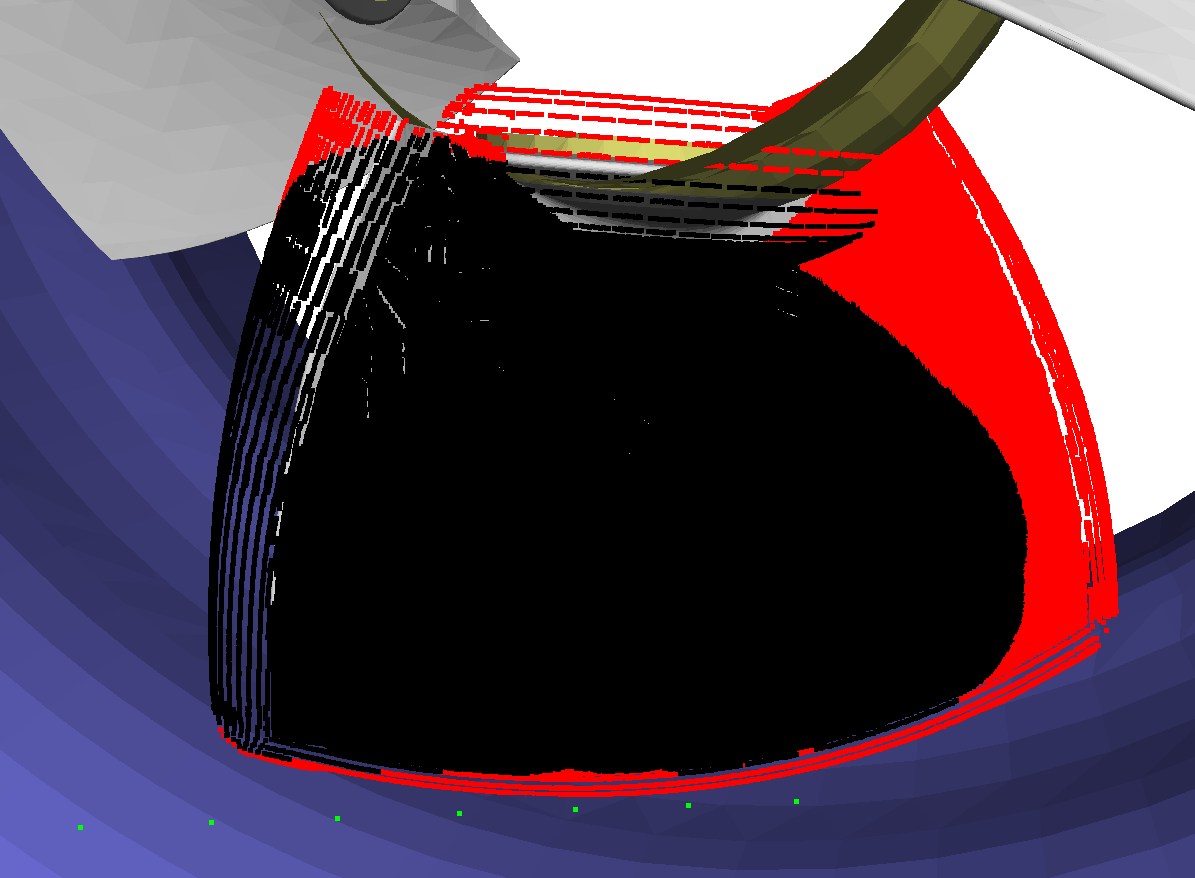
\includegraphics[width=.5\columnwidth]{figs/simcomp1_1.png}
	\caption{Simulação de revestimento completo da pá, considerando as
	restrições mecânicas da base, ângulo $0^o$ do rotor e $24^o$ da pá.}
	\label{fig::simcomp1_1}
\end{figure}

\subsubsection{Extremidade superior esquerda}
Há três possíveis soluções para revestir a extremidade superior esquerda:
elevação da base do robô; aumentar tolerância de ângulo de revestimento para
$60^o$; e rotação da turbina para $-15^o$. Como esta
região da pá tem inclinação projetada para o robô, alterar o ângulo da pá de $24^o$ para $0^o$ não favorece o
revestimento (figura~\ref{fig::simcomp1_4}). Em termos de operação, as três
medidas possuem desvantagens: rotar a turbina é complexo, visto que será
necessário realizar um procedimento para transportar os equipamentos a uma área
de segurança e fazer a recalibração; elevar o robô apresenta complexidade
mecânica, já que exige mais um grau de liberdade da base, e fazer recalibração;
aumentar a tolerância do ângulo de revestimento tem complexidade menor, mas
aumenta a perda de material de revestimento.

A figura~\ref{fig::simcomp1_5} mostra a discretização completa da pá, nas
condições em que o rotor está $-15^o$ e a pá $24^o$. Conforme o rotor é
girado no sentido horário (negativo), o revestimento na extremidade superior
esquerda da pá é completa, porém o lado direito fica prejudicado.

\begin{figure}[!ht]
	\centering	
	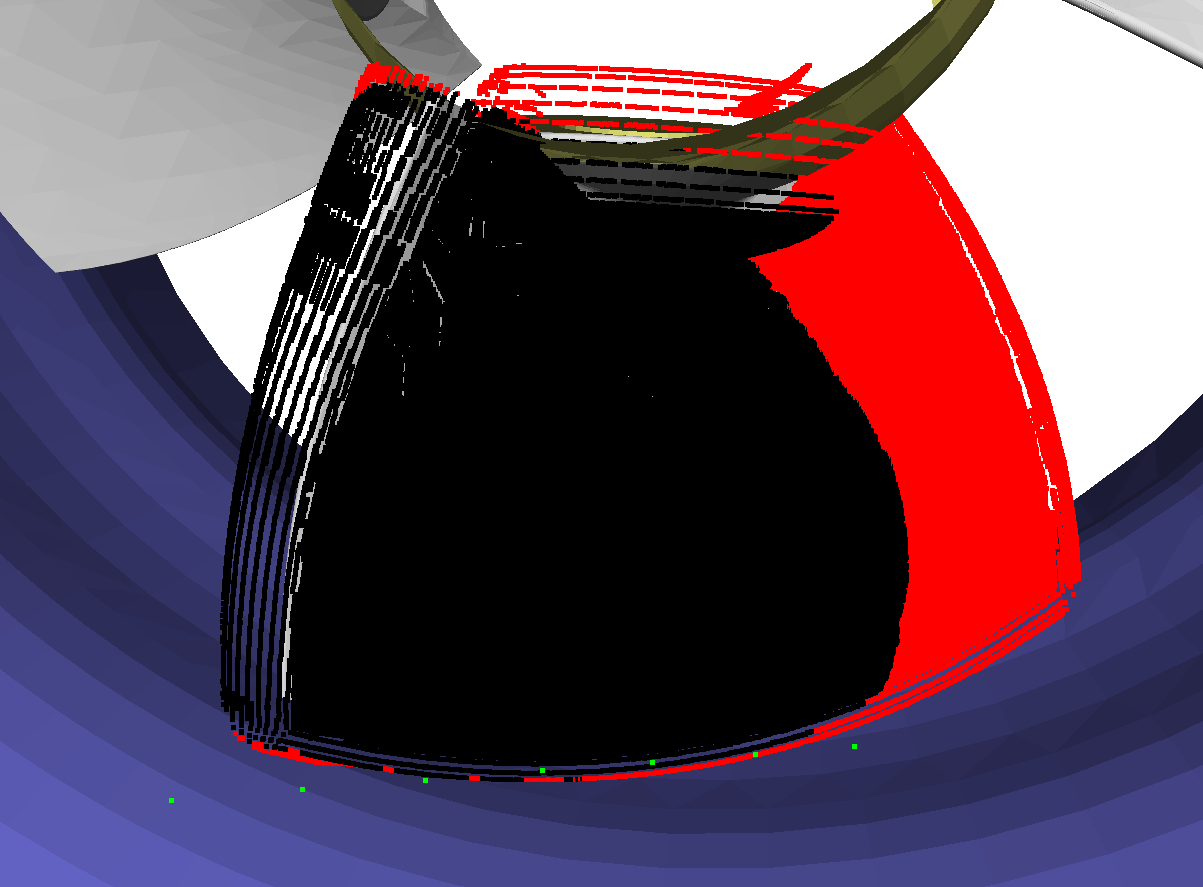
\includegraphics[width=.5\columnwidth]{figs/simcomp1_5.png}
	\caption{Simulação de revestimento completo da pá, considerando as
	restrições mecânicas da base, ângulo $-15^o$ do rotor e $24^o$ da pá.}
	\label{fig::simcomp1_5}
\end{figure}

Quando aumentamos a tolerância de ângulo de revestimento
para $60^o$, obtemos a figura\ref{fig::simcomp1_3}. A figura mostra que foi
possível revestir toda a extremidade superior esquerda, salvo pontos de colisão
com o rotor. Entretanto, é importante a base ter o grau de liberdade em $y$ para
suprir eventuais problemas de modelagem.

\begin{figure}[!ht]
	\centering	
	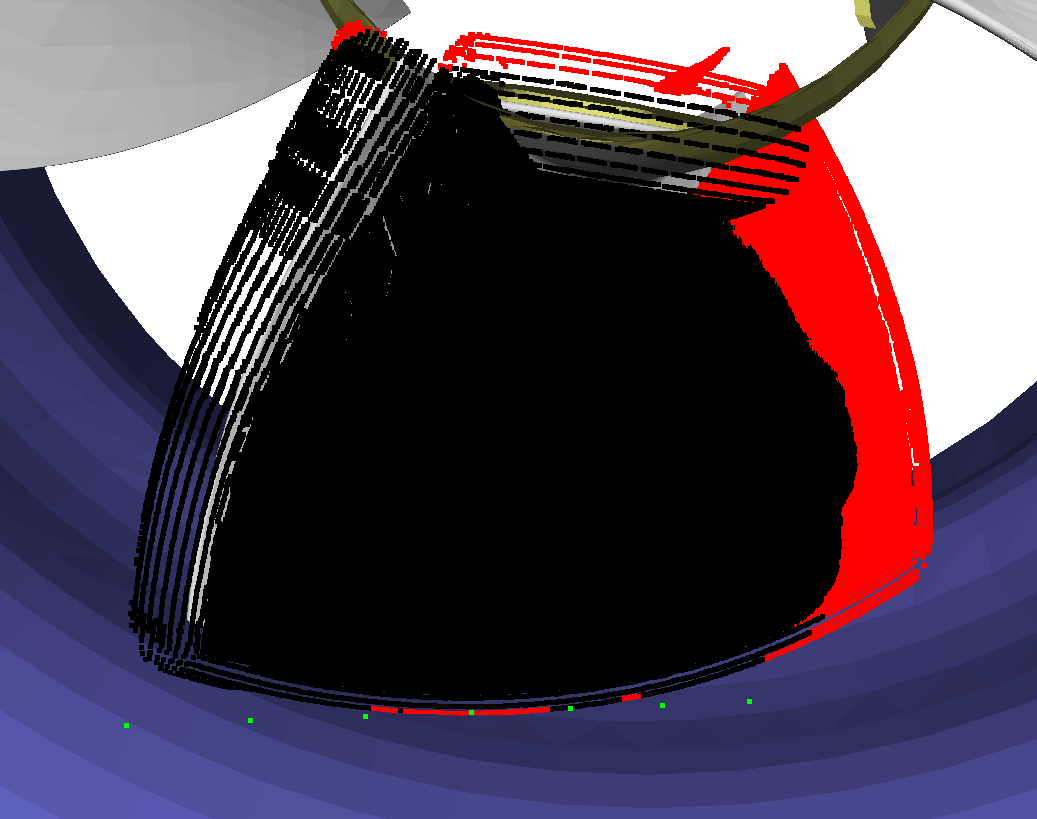
\includegraphics[width=.5\columnwidth]{figs/simcomp1_3.png}
	\caption{Simulação de revestimento completo da pá, considerando as
	restrições mecânicas da base, ângulo $0^o$ do rotor e $24^o$ da pá,
	tolerância de $60^o$ de revestimento.}
	\label{fig::simcomp1_3}
\end{figure}

Ao elevarmos a base $y+500 mm$, obtemos a figura\ref{fig::simcomp1_6}. A figura
mostra que foi possível revestir toda a extremidade superior esquerda e, ainda,
alguns pontos na lateral direita que não haviam sido revestidos. É muito
provável que este grau de liberdade da base seja projetado, a fim de o projeto
não ficar dependente dos movimentos da turbina.

\begin{figure}[!ht]
	\centering	
	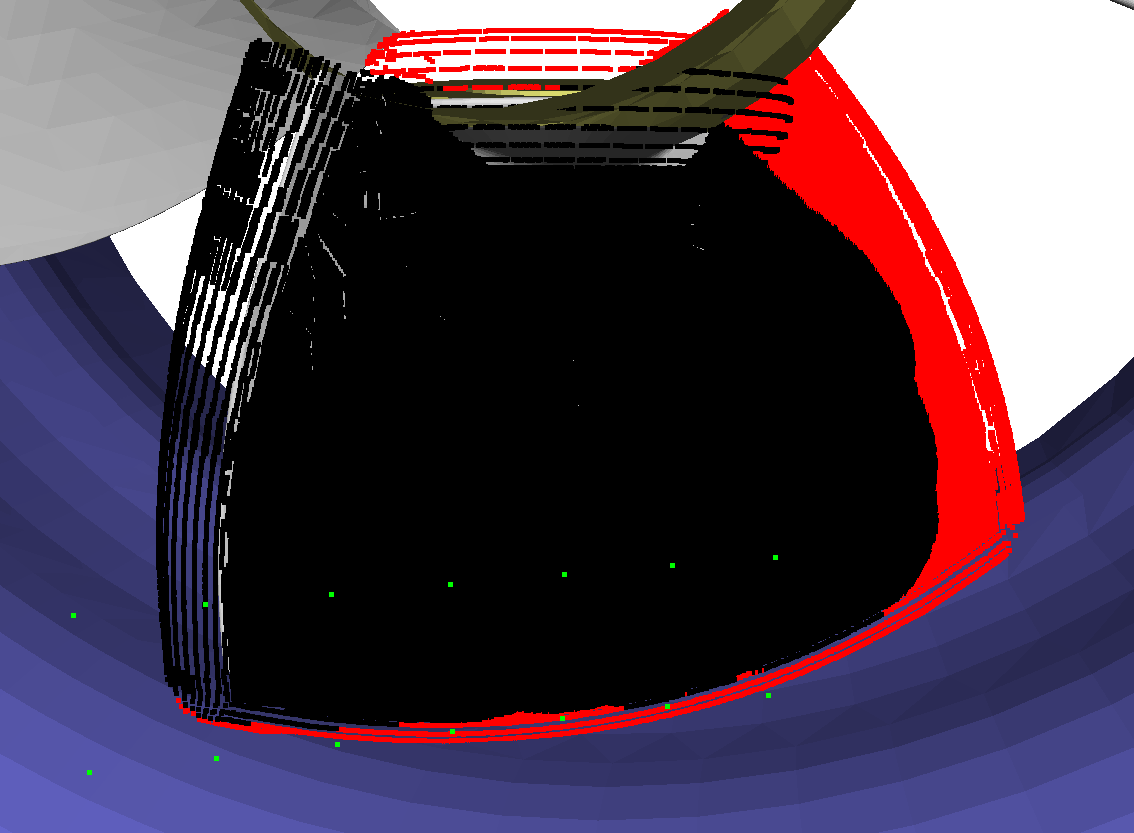
\includegraphics[width=.5\columnwidth]{figs/simcomp1_6.png}
	\caption{Simulação de revestimento completo da pá, considerando as
	restrições mecânicas da base, ângulo $0^o$ do rotor e $24^o$ da pá,
	$y+500 mm$.}
	\label{fig::simcomp1_6}
\end{figure}

\subsubsection{Lateral direita}
Em relação à lateral direita da pá, a ideia imediata é rotar a turbina,
esperando que o lado direito se aproxime do robô. Outras possibilidades é
girar a pá em seu próprio eixo para $0^o$, em vez de $24^o$. As desvantagens de
cada solução se assemelham às discutidas previamente: rotar a turbina exige
transporte dos equipamentos à área de segurança, remontagem e recalibração;
girar a pá só é possível através do circuito hidráulico e talvez não seja
possível após início da operação.

A figura~\ref{fig::simcomp1_2} mostra a discretização completa da pá, nas
condições em que o rotor está $15^o$ e a pá $24^o$. Conforme o rotor é
girado no sentido anti-horário (positivo), embora o revestimento aumente na
lateral direita da pá, a lateral esquerda e as áreas inferiores começam a ser
prejudicadas. A extremidade superior direita continua sem ser revestida, como
esperado, vide subseção~\ref{superioresquerda}.

\begin{figure}[!ht]
	\centering	
	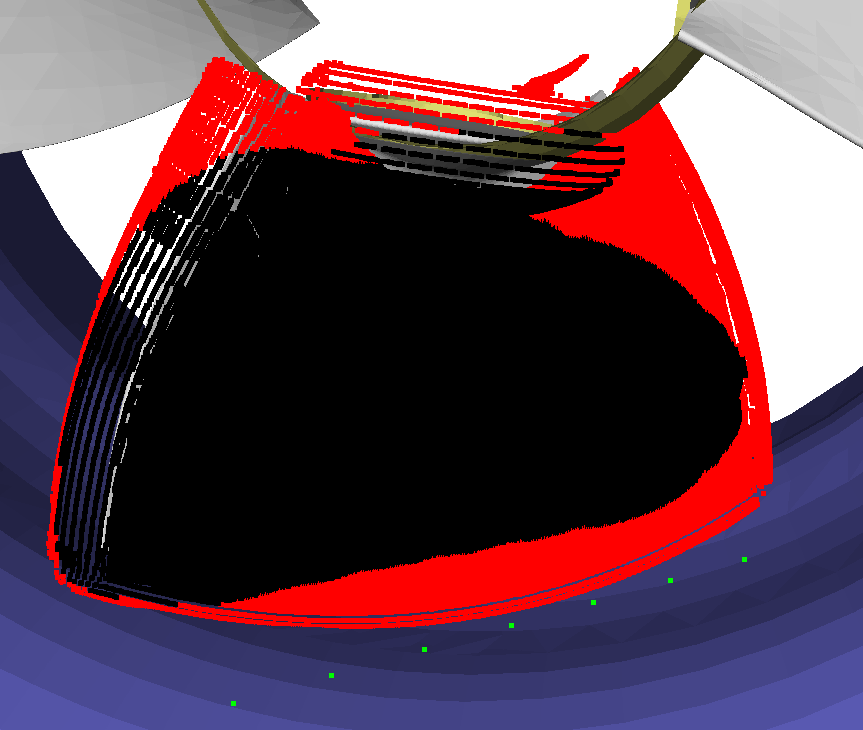
\includegraphics[width=.5\columnwidth]{figs/simcomp1_2.png}
	\caption{Simulação de revestimento completo da pá, considerando as
	restrições mecânicas da base, ângulo $15^o$ do rotor e $24^o$ da pá.}
	\label{fig::simcomp1_2}
\end{figure}

A figura~\ref{fig::simcomp1_4} mostra a discretização completa da pá, nas
condições em que o rotor está $0^o$ e a pá $0^o$. Conforme a pá é girada, o
revestimento aumenta na lateral direita e se mantém na lateral esquerda. Isso
ocorre, pois o robô se mantém longe do aro câmara no lado direito, já que o aro
ainda não está $20^o$. Esta é a melhor posição para revestimento da pá,
situação aparente ao método da Rijeza. Entretanto, esta configuração fornece
pequeno espaçamento entre pás, estreitando a passagem do robô e, muito
provavelmente, não é possível alterar esse ângulo frequentemente já que exige
funcionamento do circuito hidráulico.

\begin{figure}[!ht]
	\centering	
	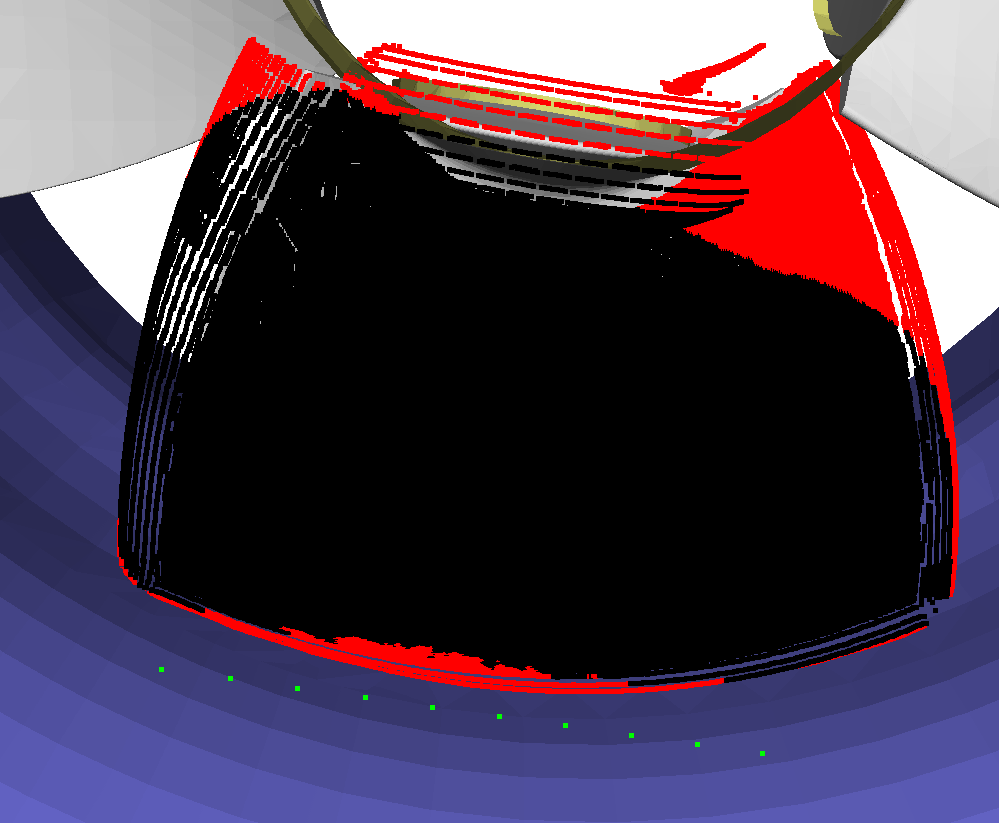
\includegraphics[width=.5\columnwidth]{figs/simcomp1_4.png}
	\caption{Simulação de revestimento completo da pá, considerando as
	restrições mecânicas da base, ângulo $0^o$ do rotor e $0^o$ da pá.}
	\label{fig::simcomp1_4}
\end{figure}

\subsubsection{Extremidade superior direita}
A extremidade superior direita requer uma nova estratégia, pois todas as
outras falharam até então: rotar turbina, girar pá, elevar o robô no trilho
$y+500 mm$. Não há possibilidade, portanto, de realizar o revestimento a partir
do trilho 2 (posicionamento). A solução encontrada até o momento é rotar a
turbina $45^o$, manter a pá em $24^o$ e posicionar o robô entre as pás, no
trilho 1 (transporte). A desvantagem logística de rotar a turbina é comum às
soluções antigas, porém, esta configuração da turbina já estava prevista para
a entrada do robô no lado do distribuidor.

A figura~\ref{fig::simcomp1_7} mostra a discretização completa da pá, nas
condições em que o rotor está $45^o$ e a pá $24^o$. O robô se encontra
com sua base nas posições destacadas em verde. Como podemos observar, nesta
configuração (robô no trilho 1), é possível revestir a extremidade
superior direita. A fim de melhor aproveitamento logístico da
operação, esta operação deve ser realizada antes da entrada completa
do robô no lado do distribuidor.

\begin{figure}[!ht]
	\centering	
	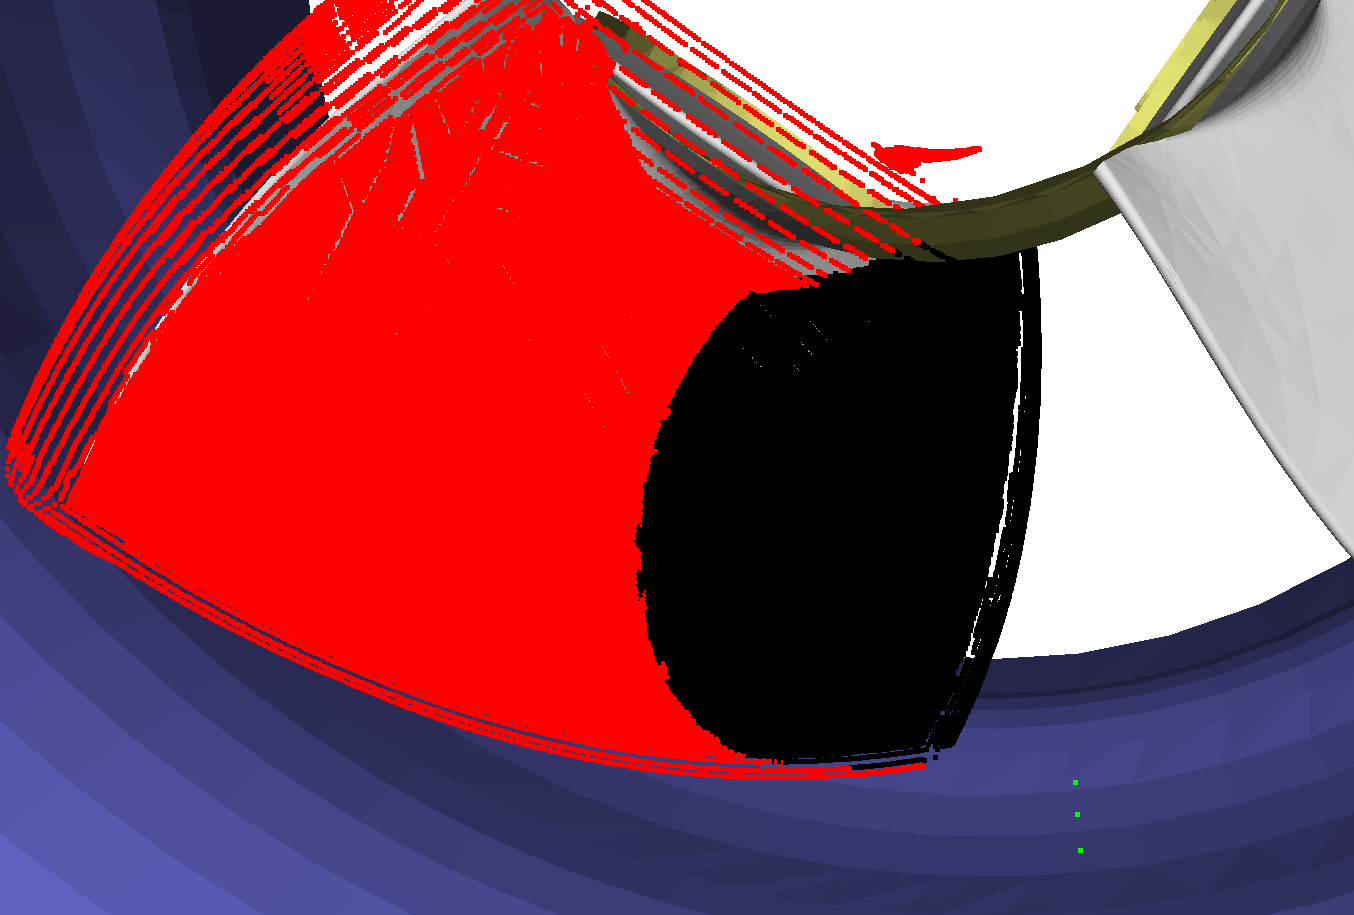
\includegraphics[width=.5\columnwidth]{figs/simcomp1_7.png}
	\caption{Simulação de revestimento completo da pá, considerando as
	restrições mecânicas da base, ângulo $45^o$ do rotor e $24^o$ da pá, robô
	entre as pás.}
	\label{fig::simcomp1_7}
\end{figure}

\subsubsection{Conclusão da simulação completa}

A simulação completa da pá mostrou diversas estratégias para o revestimento da
pá, considerando as restrições mecânicas do trilho, o ambiente modelado da
turbina, e as diversas variáveis do processo de revestimento.

A partir dos resultados das simulações, podemos concluir que é possível realizar
o revestimento completo da pá, inclusive das áreas de mais difícil acesso, como
as extremidades. O revestimento completo, no entano, requer uma extensa
logística de operação. Para cada face da pá, o robô deverá executar o
procedimento tanto no de posicionamento (trilho 2), quanto no trilho de
transporte (trilho 1), a fim de revestir a área mais complexa, extremidade
superior direita. 
